\documentclass{beamer}
\usepackage[utf8]{inputenc}
\usepackage[T1]{fontenc}
\usepackage{import}

\usetheme{default}
\usecolortheme{seahorse}
\usefonttheme{serif}

\input{../preamble}

\title{PHGN 200 --- Electromagnetism and Optics}
\subtitle{Block II: Circuits}

\author{}
\date{Block II Review Slides}

\begin{document}

\frame{\titlepage}

\begin{frame}{A Quick Introduction}

\begin{center}
Block I was all about \emph{electrostatics} --- we dealt with stationary charges.
\end{center}

\vfill

\begin{center}
Now we're in Block II, and we care about what happens when charges are mobilized in circuits.
\end{center}

\vfill

\begin{center}
So let's start at the beginning and consider \emph{moving} charges.
\end{center}

\end{frame}

\begin{frame}{Current}

Current is moving charge. Nothing more, nothing less. Mathematically, current is given by
\begin{equation*}
    I = \frac{dQ}{dt}
\end{equation*}

We can think of current as the \emph{charge per unit time} passing a given point. Current is measured in coulombs-per-second, or \textbf{amperes} (A):
\begin{equation*}
    \SI{1}{\ampere} = \SI{1}{\coulomb/\second}
\end{equation*}

\end{frame}

\begin{frame}{A Historical Confusion --- Blame Ben Franklin}

In practice, it is ordinarily the negatively charged electrons that do the moving --- in the direction \emph{opposite} to the electric current.

\begin{figure}[H]
\centering
\begin{circuitikz}
    \draw (0,0) to[battery,i>=$I$] (0,3);
    \draw (0,3) to (1.5,3) node[label={[font=\tiny]above:$\textcolor{BLUE}{\longleftarrow \text{electron flow} \longleftarrow}$}] {} to (3,3);
    \draw (3,3) to[resistor,i>=$I$] (3,0);
    \draw (3,0) to (0,0);
    \draw (3,0) to (1.5,0) node[label={[font=\tiny]below:$\textcolor{BLUE}{\longrightarrow \text{electron flow} \longrightarrow}$}] {} to (0,0);
\end{circuitikz}
\end{figure}

To avoid complicating things, we often pretend it's the positive charges that move. That is, we don't care about the direction the electrons move (and instead only focus on the flow of positive charges).

\end{frame}

\begin{frame}{Worked Example --- Finding how much Charge Passed a Given Point}

$\blacktriangleright$ Suppose the current at some point in a wire is given by the function $I(t) = I_o e^{-t/2}$, where $I_o = \SI{2.2}{\ampere}$.

\begin{figure}[H]
\centering
\begin{tikzpicture}[scale=0.6]
\begin{axis}[axis lines = center, xlabel = $t$, ylabel = {$I(t)$}]
% \addplot[domain=0:10, samples=200, color=blue] {-0.4*sin(1.7453*deg(x))+2};
\addplot[domain=0:16, samples=200, color=blue] {2.2*exp(-x/2)};
\end{axis}
\end{tikzpicture}
\end{figure}

How much charge passes through that point in the wire?

\end{frame}

\begin{frame}{Worked Example --- Finding how much Charge Passed a Given Point}

\textit{Solution.} Current is defined by $I = \frac{dQ}{dt}$. This implies that a differential amount of charge is given by
\begin{equation*}
    dQ = I\ dt
\end{equation*}

Then we can find the \emph{total} amount of charge by integrating:
\begin{equation*}
    Q = \int dQ = \int I\ dt
\end{equation*}
    
\end{frame}

\begin{frame}{Worked Example --- Finding how much Charge Passed a Given Point}

So we know that integrating $I$ with respect to time gives us charge. But what time do we integrate over?

\vfill

We're looking for the \emph{total charge} that goes through that point in the circuit. So we might as well integrate over all time.

\vfill

\textit{Pause and Ponder:} Where would we see a physical example of such a current?

\end{frame}

\begin{frame}{Worked Example --- Finding how much Charge Passed a Given Point}

Integrating, we get
\begin{align*}
    Q = \int dQ &= \int I\ dt \\
                &= \int_{0}^{\infty} \left( I_o e^{-t/2} \right)\ dt \\
                &= I_o \left( -2 e^{-t/2} \right) \bigg|_{0}^{\infty} \\
                &= \left( \SI{2}{\second} \right) I_o
\end{align*}

Thus, the total charge that passes through that point in the circuit is
\begin{equation*}
    \left( \SI{2}{\second} \right) \left( \SI{2.2}{\ampere} \right) = \boxed{ \SI{4.4}{\coulomb} = Q } \blacktriangleleft
\end{equation*}

\end{frame}

\begin{frame}{Another Definition of Current}

Consider a some conductor where the density of charge-carriers is $n$ (and each has charge $q$), the cross-sectional area is $A$, and the drift velocity of the charge carriers is $v_d$. Then the current is
\begin{equation*}
    I = n \left|q\right| v_d A
\end{equation*}

If the charge carriers are electrons, then their charge is $e_f = \SI{1.602e-19}{\coulomb}$, and the current is
\begin{equation*}
    I = n e_f v_d A
\end{equation*}

Additionally, we can consider just the \emph{current per unit area} which is known as the current density:
\begin{equation*}
    J = \frac{I}{A} = n q v_d
\end{equation*}

\begin{center}
(Current density will come back in Block III.)
\end{center}

\end{frame}

\begin{frame}{Voltage}

So we've established what \emph{current} is. It's nothing more than \emph{moving charges}. But how did we get these charges moving in the first place? They certaintly don't move on their own, right?

\vfill

Voltage is defined to be the amount of \emph{energy per unit charge}. The change in energy by some charge $q$ in moving from point $a$ to point $b$ is

\begin{equation*}
    \Delta U = q \left( V_b - V_a \right) = q \Delta V
\end{equation*}

\vfill

(The energy that actually drives charges can come from a battery --- in which case a chemical reaction is supplying the energy.)

\end{frame}

\begin{frame}{Resistance}

Resistance is a way of quantifying how much effort it takes to move charge across less-than-perfect conductors. Experimentally, we find that, for most materials

\begin{equation*}
    R = \frac{\varrho\ L}{A} \quad \implies \quad dR = \frac{\varrho\ dL}{A}
\end{equation*}

where $\varrho$ is the electrical resistivity, measured in ohm-meter (\si{\ohm\cdot\metre}), $L$ is the length of the resistor, and $A$ is the cross-sectional area.
    
\end{frame}

\begin{frame}{Worked Example --- Resistance of a Goofy Resistor}

$\blacktriangleright$ Suppose a solid ``lampshade'' has height $h$ and base radii $a$ and $a/2$. Wires are attached to the ends of the ``lampshade'' as shown below:

\begin{figure}[H]
\centering
\includegraphics[height=0.5\textheight]{figures/half.png}
\end{figure}

Given that the cone has resistivity $\varrho$, what is the resistance of such a configuration?

\end{frame}

\begin{frame}{Worked Example --- Resistance of a Goofy Resistor}

\textit{Solution.} We want to find the resistance of some goofy ``lampshade'' resistor. As such, we'll want to start with the familiar expression for differential resistance:

\begin{equation*}
    dR = \frac{\varrho\ dL}{A}
\end{equation*}

This is our governing equation. Now let's build it up.

\end{frame}

\begin{frame}{Worked Example --- Resistance of a Goofy Resistor}

For the sake of simplicity, let's make the axis of the ``lampshade'' the $x$-axis, with the smaller base at $x = 0$.

\begin{figure}[H]
\centering
\includegraphics[height=0.5\textheight]{figures/lamponx.png}
\end{figure}

Then $dL$ --- the differential length through the resistor --- is $dx$.

\end{frame}

\begin{frame}{Worked Example --- Resistance of a Goofy Resistor}

What about the area? The area in the expression $dR = \frac{\varrho\ dL}{A}$ refers to the \emph{cross-sectional} area that the current ``sees'' when moving through the resistor. In our case: circles!

\begin{figure}[H]
\centering
\includegraphics[height=0.5\textheight]{figures/lampcirc.png}
\end{figure}

And we know the area of a circle is $\pi r^2$. But what \emph{exactly} is the radius?

\end{frame}

\begin{frame}{Worked Example --- Resistance of a Goofy Resistor}

Let's look at the ``lampshade'' from the side.

\begin{figure}[H]
\centering
\includegraphics[height=0.3\textheight]{figures/whatradius.png}
\end{figure}

We can deduce that the radius $r$ as a function of the position $x$ along the $x$-axis is
\begin{equation*}
    r = \frac{a}{2h} x + \frac{a}{2} = \frac{a \left(x + h\right)}{2h}
\end{equation*}

And thus the \emph{cross-sectional} area as a function of the position $x$ along the $x$-axis is
\begin{equation*}
    A = \pi \left[ \frac{a \left(x + h\right)}{2h} \right]^2 = \frac{\pi a^2 \left(x + h\right)^2}{4h^2}
\end{equation*}

\end{frame}

\begin{frame}{Worked Example --- Resistance of a Goofy Resistor}

All that's left is to put everything together and integrate. We have
\begin{align*}
    R = \int dR &= \int_{0}^{h} \frac{(4h^2) \varrho\ dx}{\pi a^2\ \left( x + h \right)^2} \\
                &= \frac{(4h^2) \varrho}{\pi a^2} \int_{0}^{h} \frac{dx}{\left(x + h\right)^2} \\
                &= \frac{(4h^2) \varrho}{\pi a^2} \left( -\frac{1}{x + h} \right) \bigg|_{0}^{h}
\end{align*}

So in conclusion, the resistance of the entire configuration is
\begin{equation*}
    \boxed{R = \frac{2 h \varrho}{\pi a^2}} \blacktriangleleft
\end{equation*}

\end{frame}

\begin{frame}{Resistors in Series}

Resistors can be arranged in series:

\begin{figure}[H]
\centering
\begin{circuitikz}
    \draw (0,0) to[R,l^=$R_1$] (2,0);
    \draw (2,0) to[R,l^=$R_2$] (4,0);
    \draw (4,0) to[R] (6,0);
    \draw (6,0) to[R,l^=$R_n$] (8,0);
\end{circuitikz}
\end{figure}

\begin{center}
Resistors in series carry the same current.
\end{center}

\vfill

The equivalent resistance of $n$ resistors in series is
\begin{equation*}
    R_{\text{eq}} = R_1 + R_2 + \cdots + R_n
\end{equation*}

\end{frame}

\begin{frame}{Resistors in Parallel}

Resistors can also be arranged in parallel:

\begin{figure}[H]
\centering
\begin{circuitikz}
    \draw (0,0) to (6,0);
    \draw (0,0) to[R,l^=$R_1$] (0,2);
    \draw (2,0) to[R,l^=$R_2$] (2,2);
    \draw (4,0) to[R] (4,2);
    \draw (6,0) to[R,l^=$R_n$] (6,2);
    \draw (0,2) to (6,2);
\end{circuitikz}
\end{figure}

\begin{center}
Resistors in parallel are subject to the same voltage drop.
\end{center}

\vfill

The equivalent resistance of $n$ resistors in parallel is
\begin{gather*}
    \frac{1}{R_{\text{eq}}} = \frac{1}{R_1} + \frac{1}{R_2} + \cdots + \frac{1}{R_n} \\
    \implies R_{\text{eq}} = \left( \frac{1}{R_1} + \frac{1}{R_2} + \cdots + \frac{1}{R_n} \right)^{-1}
\end{gather*}

\end{frame}

\begin{frame}{Ohm's Law}

So we know that current $I$ is nothing more than moving charges. In a circuit, a difference in voltage $\Delta V$ (say, from a battery) drives the movement of these charges. And since these charges probably move across less-than-perfect conductors, they encounter a resistance $R$. 

\vfill

These quantities are related by \emph{Ohm's Law}, which reads
\begin{equation*}
    \Delta V = IR
\end{equation*}

In other words, the voltage difference $\Delta V$ across a load with resistance $R$ is proportional to the current $I$.

\end{frame}

\begin{frame}{Energy and Power in Circuits}

The power dissipated by a circuit component is
\begin{equation*}
    P = I \left( \Delta V \right)
\end{equation*}

For \emph{ohmic} material (that is, where Ohm's law applies), this becomes
\begin{equation*}
    P = I \left( \Delta V \right) = I^2 R = \frac{\left( \Delta V \right)^2}{R}
\end{equation*}

Now say I want to calculate the energy dissipated by some circuit component over a period of time from $t_i$ to $t_f$. Power is defined as the time derivative of energy so 
\begin{gather*}
    P \equiv \frac{dU}{dt} \quad \implies \quad dU = P\ dt \\
    \implies U = \int_{t_i}^{t_f} P\ dt
\end{gather*}

\end{frame}

\begin{frame}{Kirchhoff's Current Law}

The sum of the currents entering a junction is equal to the sum of the currents leaving a junction:

\begin{equation*}
    \underbrace{\hspace{2em}\sum I_{\text{in}} = \sum I_{\text{out}}\hspace{2em}}_{\parbox[c]{0.8\textwidth}{\begin{center} This is a statement of charge conservation \end{center}}}
\end{equation*}

\vfill

Note that a junction is any place on a circuit where three or more wires meet.

\end{frame}

\begin{frame}{Kirchhoff's Voltage Law}

The sum of voltage drops around a closed loop is zero:

\begin{equation*}
    \underbrace{\hspace{2em}\sum \Delta V = 0 \quad \text{for any closed loop}\hspace{2em}}_{\parbox[c]{0.8\textwidth}{\begin{center} This is a statement of energy conservation \end{center}}}
\end{equation*}

\end{frame}

\begin{frame}{How to Use Kirchhoff's Voltage Law}

For any closed loop in a circuit: 

\begin{enumerate}

\item[(1)] Choose a starting location and go all the way around the loop, returning to where you started. Go either \emph{clockwise} or \emph{counterclockwise} --- but be consistent!

\item[(2)] As you encounter a circuit element (whether that's a battery, emf source, capacitor, or a resistor) decide whether there's a \textcolor{GREENE}{positive} or \textcolor{RED}{negative} contribution to $\Delta V$ according to the following sign conventions:

\begin{itemize}

\item[$\bullet$] Crossing a battery (or emf source) from the \emph{negative} terminal to the \emph{positive} terminal gives a \textcolor{GREENE}{positive contribution to $\Delta V$}

\item[$\bullet$] Crossing a capacitor from the \emph{negative} plate to the \emph{positive} plate gives a \textcolor{GREENE}{positive contribution to $\Delta V$}

\item[$\bullet$] Crossing a resistor in the direction of \emph{positive current flow} gives a \textcolor{RED}{negative contribution to $\Delta V$}

\item[$\bullet$] Vice versa for all the above

\end{itemize}

\end{enumerate}

\end{frame}

\begin{frame}{Worked Example --- Kirchhoff Analysis}

$\blacktriangleright$ The following diagram shows a circuit where: $R_1 = \SI{8.0}{\ohm}$, $R_2 = \SI{7.0}{\ohm}$, $R_3 = \SI{4.0}{\ohm}$, $V_1 = \SI{4.2}{\volt}$, $V_2 = \SI{18.0}{\volt}$, and $V_3 = \SI{4.5}{\volt}$. What is the value of $I_1$?

\begin{figure}[H]
\centering
\begin{circuitikz}
    \draw (0,0) to[battery,l^=$V_1$] (0,1.3);
    \draw (0,0.9) to[resistor,l^=$R_1$,i>=$\textcolor{BLUE}{I_1}$] (0,3);
    \draw (0,3) to[battery,invert,l^=$V_2$] (0,4);
    \draw (0,0) to (3,0);
    \draw (0,4) to (3,4);
    \draw (3,0) to[resistor,l^=$R_2$,i>=$\textcolor{BLUE}{I_2}$] (3,4);
    \draw (3,0) to (6,0);
    \draw (3,4) to (6,4);
    \draw (6,0) to[battery,invert,l^=$V_3$,i>=$\textcolor{BLUE}{I_3}$] (6,2.4);
    \draw (6,2) to[resistor,l^=$R_3$] (6,4);
    % \draw (0,0) to[battery,i>=$I$] (0,3);
    % \draw (0,3) to (1.5,3) node[label={[font=\tiny]above:$\textcolor{BLUE}{\longleftarrow \text{electron flow} \longleftarrow}$}] {} to (3,3);
\end{circuitikz}
\end{figure}

\end{frame}

\begin{frame}{Worked Example --- Kirchhoff Analysis}

\textit{Solution.} Let's start with the junction equations. Kirchhoff's Junction Law reads

\begin{equation*}
    \sum I_{\text{in}} = \sum I_{\text{out}}
\end{equation*}

And there are two junctions on our circuit:

\begin{figure}[H]
\centering
\begin{circuitikz}[scale=1.0]
    \draw (0,0) to[battery,l^=$V_1$] (0,1.3);
    \draw (0,0.9) to[resistor,l^=$R_1$,i>=$\textcolor{BLUE}{I_1}$] (0,3);
    \draw (0,3) to[battery,invert,l^=$V_2$] (0,4);
    \draw (0,0) to (3,0);
    \draw (0,4) to (3,4);
    \draw (3,0) to[resistor,l^=$R_2$,i>=$\textcolor{BLUE}{I_2}$] (3,4);
    \draw (3,0) to (6,0);
    \draw (3,4) to (6,4);
    \draw (6,0) to[battery,invert,l^=$V_3$,i>=$\textcolor{BLUE}{I_3}$] (6,2.4);
    \draw (6,2) to[resistor,l^=$R_3$] (6,4);
    \draw (3,3) to[short,-*,color=red] (3,4) node[label={[font=\small]above:$\textcolor{RED}{\text{Top Junction}}$}] {} to (3,3);
    \draw (3,1) to[short,-*,color=red] (3,0) node[label={[font=\small]below:$\textcolor{RED}{\text{Bottom Junction}}$}] {} to (3,1);
\end{circuitikz}
\end{figure}

\end{frame}

\begin{frame}{Worked Example --- Kirchhoff Analysis}

For the top junction, we have:
\begin{equation*}
    \underbrace{\hspace{0.2em} I_1 + I_2 + I_3 \hspace{0.2em}}_{\parbox[c]{0.4\textwidth}{\begin{center} \vspace{-0.7em} \tiny All three currents entering junction \end{center}}} \hspace{-2em} = \hspace{-3em} \overbrace{\hspace{1.4em} 0 \hspace{1.4em}}^{\parbox[c]{0.4\textwidth}{\begin{center} \tiny No currents leaving \vspace{-1em} \end{center}}}
\end{equation*}

And for the bottom junction:
\begin{equation*}
    \underbrace{\hspace{1.4em} 0 \hspace{1.4em}}_{\parbox[c]{0.2\textwidth}{\begin{center} \vspace{-0.7em} \tiny No currents entering junction \end{center}}} \hspace{-1em} = \hspace{-2em} \overbrace{\hspace{0.2em} I_1 + I_2 + I_3 \hspace{0.2em}}^{\parbox[c]{0.4\textwidth}{\begin{center} \tiny All three currents leaving \vspace{-1em} \end{center}}}
\end{equation*}

These two equations are saying the same thing, and we don't need that redundancy. So the junction equation is:
\begin{equation*}
    I_1 + I_2 + I_3 = 0
\end{equation*}

\end{frame}

\begin{frame}{Worked Example --- Kirchhoff Analysis}

Now it's time to look at the loop equations. (Let's go clockwise)

\begin{figure}[H]
\centering
\begin{circuitikz}
    \draw (0,0) to[battery,l^=$V_1$] (0,1.3);
    \draw (0,0.9) to[resistor,l^=$R_1$,i>=$\textcolor{BLUE}{I_1}$] (0,3);
    \draw (0,3) to[battery,invert,l^=$V_2$] (0,4);
    \draw (0,0) to (3,0);
    \draw (0,4) to (3,4);
    \draw (3,0) to[resistor,l^=$R_2$,i>=$\textcolor{BLUE}{I_2}$] (3,4);
    \draw (3,0) to (6,0);
    \draw (3,4) to (6,4);
    \draw (6,0) to[battery,invert,l^=$V_3$,i>=$\textcolor{BLUE}{I_3}$] (6,2.4);
    \draw (6,2) to[resistor,l^=$R_3$] (6,4);
\end{circuitikz}
\end{figure}

For the loop on the left:

\begin{equation*}
    +V_1 - I_1 R_1 - V_2 + I_2 R_2 = 0
\end{equation*}

And for the loop on the right:

\begin{equation*}
    -I_2 R_2 + I_3 R_3 + V_3 = 0
\end{equation*}

\end{frame}

\begin{frame}{Worked Example --- Kirchhoff Analysis}

Let's take a look at what happens when we add the equations for the left and right loops:

\begin{align*}
    V_1 - I_1 R_1 - V_2 + \cancel{I_2 R_2} &= 0 \\
    (+) \qquad \cancel{-I_2 R_2} + I_3 R_3 + V_3 &= 0 \\
    \cline{1-2}
    V_1 - I_1 R_1 - V_2 + I_3 R_3 + V_3 &= 0
\end{align*}

\begin{center}
This is exactly the equation for the big loop (that encompasses the whole circuit)!
\end{center}

\vfill

This tells us that the big loop equation is redundant so we won't include it. (After all, we already have three equations for our three unknowns $I_1$, $I_2$, and $I_3$.)

\end{frame}

\begin{frame}{Worked Example --- Kirchhoff Analysis}

So to summarize what we have so far:
\begin{align*}
    \text{Left loop:}&& V_1 - I_1 R_1 - V_2 + I_2 R_2 &= 0 \\
    \text{Right loop:}&& -I_2 R_2 + I_3 R_3 + V_3 &= 0 \\
    \text{Junction:}&& I_1 + I_2 + I_3 &= 0
\end{align*}

\vfill

Now we just have to solve for $I_1$. To do so, let's solve for $I_2$ and $I_3$ in terms of $I_1$ and plug everything into the junction equation.

\end{frame}

\begin{frame}{Worked Example --- Kirchhoff Analysis}

Solving the left loop equation for $I_2$ gives
\begin{equation*}
    I_2 = \frac{I_1 R_1 + V_2 - V_1}{R_2}
\end{equation*}

And solving the right loop equation for $I_3$ gives
\begin{equation*}
    I_3 = \frac{I_2 R_2 - V_3}{R_3}
\end{equation*}

Into which we can sub in what we just found for $I_2$:
\begin{equation*}
    I_3 = \frac{\overbrace{\left( \frac{I_1 R_1 + V_2 - V_1}{R_2} \right)}^{I_2} R_2 - V_3}{R_3} = \frac{I_1 R_1 + V_2 - V_1 - V_3}{R_3}
\end{equation*}

Awesome. Now we have $I_2$ and $I_3$ in terms of $I_1$.

\end{frame}

\begin{frame}{Worked Example --- Kirchhoff Analysis}

Now let's plug everything into the junction equation:
\begin{equation*}
    I_1 + \overbrace{\left( \frac{I_1 R_1 + V_2 - V_1}{R_2} \right)}^{I_2} + \overbrace{\left( \frac{I_1 R_1 + V_2 - V_1 - V_3}{R_3} \right)}^{I_3} = 0
\end{equation*}

And, after a bit of tedious work, we get
\begin{equation*}
    I_1 = \frac{\frac{V_1 - V_2}{R_2} + \frac{V_1 + V_3 - V_2}{R_3}}{1 + \frac{R_1}{R_2} + \frac{R_1}{R_3}} = \boxed{\frac{\left( R_2 + R_3 \right) \left( V_1 - V_2 \right) + R_2 V_3}{R_2 R_3 + R_1 \left( R_2 + R_3 \right)} = I_1}
\end{equation*}

Plugging things in gives us a current of \SI{-1.037}{\ampere}. (The negative sign means the actual current is in the opposite direction of the drawn arrow.) $\blacktriangleleft$

\end{frame}


\begin{frame}{Capacitors}

\emph{Capacitance} is defined as the amount of charge $Q$ stored per unit voltage applied:
\begin{equation*}
    C \equiv \frac{Q}{\Delta V}
\end{equation*}

Capacitance is measured in \textbf{farads} (F):
\begin{equation*}
    \SI{1}{\farad} = \SI{1}{\coulomb/\volt}
\end{equation*}

A \emph{capacitor} is a device with two electrodes, each storing equal and opposite amounts of charge, separated by an insulator (vacuum or dielectric). Capacitance is always positive.

\end{frame}

\begin{frame}{Energy in Capacitors}

Capacitors store energy in the form of electric fields. For a capacitor with capacitance $C$ and potential difference $\Delta V$, the energy stored is
\begin{equation*}
    U_c = \frac{1}{2} C \left( \Delta V \right)^2
\end{equation*}

We can also express the energy in a capacitor in terms of its charge $Q$. We have
\begin{equation*}
    C = \frac{Q}{\Delta V} \quad \implies \quad \Delta V = \frac{Q}{C}
\end{equation*}

Substituting this above, we get
\begin{equation*}
    U = \frac{1}{2} C \left( \frac{Q}{C} \right)^2 = \frac{1}{2} \frac{Q^2}{C}
\end{equation*}

\end{frame}

\begin{frame}{Capacitors in Series}

Capacitors can be arranged in series:

\begin{figure}[H]
\centering
\begin{circuitikz}
    \draw (0,0) to[C,l^=$C_1$] (2,0);
    \draw (2,0) to[C,l^=$C_2$] (4,0);
    \draw (4,0) to[C] (6,0);
    \draw (6,0) to[C,l^=$C_n$] (8,0);
\end{circuitikz}
\end{figure}

Capacitors in series store the same charge.

\vfill

The equivalent capacitance of $n$ capacitors in series is
\begin{gather*}
    \frac{1}{C_{\text{eq}}} = \frac{1}{C_1} + \frac{1}{C_2} + \cdots + \frac{1}{C_n} \\
    \implies C_{\text{eq}} = \left( \frac{1}{C_1} + \frac{1}{C_2} + \cdots + \frac{1}{C_n} \right)^{-1}
\end{gather*}
    
\end{frame}

\begin{frame}{Capacitors in Parallel}

Capacitors can also be arranged in parallel:
\begin{figure}[H]
\centering
\begin{circuitikz}
    \draw (0,0) to (6,0);
    \draw (0,0) to[C,l^=$C_1$] (0,2);
    \draw (2,0) to[C,l^=$C_2$] (2,2);
    \draw (4,0) to[C] (4,2);
    \draw (6,0) to[C,l^=$C_n$] (6,2);
    \draw (0,2) to (6,2);
\end{circuitikz}
\end{figure}

Capacitors in parallel are subject to the same voltage drop.

\vfill

The equivalent capacitance of $n$ capacitors in parallel is
\begin{equation*}
    C_{\text{eq}} = C_1 + C_2 + \cdots + C_n
\end{equation*}
    
\end{frame}

\begin{frame}{Worked Example --- Deriving the Capacitance of a Parallel Plate Capacitor}

$\blacktriangleright$ According to the equation sheet, the capacitance of a parallel-plate capacitor with plate separation distance $d$ and plate area $A$ is
\begin{equation*}
    C = \frac{\epsilon_o A}{d}
\end{equation*}

Derive this expression.
    
\end{frame}

\begin{frame}{Worked Example --- Deriving the Capacitance of a Parallel Plate Capacitor}

\textit{Solution.} So we have a parallel plate capacitor. Let's assume that $d \ll A$ (that is, the plate separation distance is small compared to the area of the plates).

\vfill

This is a pretty good approximation, and it allows us to treat the plates of the capacitor as two infinite sheets of charge. The electric field produced by a single infinite sheet of charge is $\frac{\sigma}{2\epsilon_o}$, so the electric field in the capacitor is
\begin{equation*}
    E_{\text{parallel plate cap}} = 2 \left( \frac{\sigma}{2\epsilon_o} \right) = \frac{\sigma}{\epsilon_o}.
\end{equation*}

\end{frame}

\begin{frame}{Worked Example --- Deriving the Capacitance of a Parallel Plate Capacitor}

Recall that $\sigma$ is the surface charge density, which is uniformly distributed on the capacitor's plates:
\begin{equation*}
    E_{\text{parallel plate cap}} = \frac{\overbrace{\left( Q / A \right)}^{\sigma}}{\epsilon_o} = \frac{Q}{\epsilon_o\ A}.
\end{equation*}

We can integrate to find the magnitude of the potential difference across the plates of the capacitor:
\begin{align*}
    \big| \Delta V \big| &= \left| -\int \vec{E} \cdot d\vec{\ell} \right| = \int \vec{E} \cdot d\vec{\ell}
\end{align*}

we know the electric field, and we're integrating across the plates of the capacitor (so our bounds of integration are from $0$ to $d$).
    
\end{frame}

\begin{frame}{Worked Example --- Deriving the Capacitance of a Parallel Plate Capacitor}

So the magnitude of the potential difference is
\begin{align*}
    \big| \Delta V \big| &= \int \vec{E} \cdot d\vec{\ell} = \int_0^d \underbrace{\left( \frac{Q}{\epsilon_o A} \right)}_{E}\ d{\ell} = \left( \frac{Q}{\epsilon_o A} \right) {\int_0^d d\ell} = \frac{Q\ d}{\epsilon_o\ A}
\end{align*}

Note that the electric field is constant in space, so it could be pulled out of the integral. Finally, we can find capacitance by invoking the definition of capacitance:
\begin{equation*}
    \boxed{C = \frac{Q}{\Delta V} = \frac{\cancel{Q}}{\frac{\cancel{Q}\ d}{\epsilon_o\ A}} = \frac{\epsilon_o A}{d}} \blacktriangleleft
\end{equation*}

\end{frame}

\begin{frame}{Dielectrics}

Sometimes, the space between a capacitor's electrodes is filled with some insulating material (other than a vacuum). Such materials are called \emph{dielectrics}, and serve to increase the capacitance of the capacitor.

\vfill

Dielectrics increase the capacitance of a capacitor by a factor $\kappa$, where $\kappa$ is the dielectric constant.

\vfill

\begin{center}
But how though?
\end{center}

\end{frame}

\begin{frame}{Dielectrics}

A capacitor, by itself, creates an electric field between its plates. Shown below is a parallel plate capacitor, with electric field lines going from the positive electrode to the negative electrode.

\begin{figure}[H]
\captionsetup{width=0.8\textwidth,labelfont={color=black,bf},textfont={color=black}}
\centering
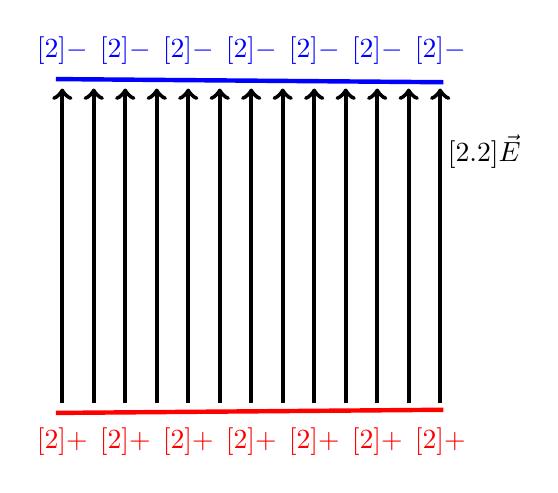
\begin{tikzpicture}[xscale=0.4,yscale=0.4]
    \draw[black, ultra thick, ->] (-6.2,-5) -- (-6.2,5);
    \draw[black, ultra thick, ->] (-5.2,-5) -- (-5.2,5);
    \draw[black, ultra thick, ->] (-4.2,-5) -- (-4.2,5);
    \draw[black, ultra thick, ->] (-3.2,-5) -- (-3.2,5);
    \draw[black, ultra thick, ->] (-2.2,-5) -- (-2.2,5);
    \draw[black, ultra thick, ->] (-1.2,-5) -- (-1.2,5);
    \draw[black, ultra thick, ->] (-0.2,-5) -- (-0.2,5);
    \draw[black, ultra thick, ->] (0.8,-5) -- (0.8,5);
    \draw[black, ultra thick, ->] (1.8,-5) -- (1.8,5);
    \draw[black, ultra thick, ->] (2.8,-5) -- (2.8,5);
    \draw[black, ultra thick, ->] (3.8,-5) -- (3.8,5);
    \draw[black, ultra thick, ->] (4.8,-5) -- (4.8,5);
    \draw[black, ultra thick, ->] (5.8,-5) -- (5.8,5);
    \node[black] at (7.2,3) {$\Scale[2.2]{\vec{E}}$};
    \draw[red, ultra thick] (-6.4,-5.3) -- (5.9,-5.2);
    \draw[blue, ultra thick] (-6.4,5.3) -- (5.9,5.2);
    \node[blue] at (-6.2,6.2) {$\Scale[2]{-}$};
    \node[blue] at (-4.2,6.2) {$\Scale[2]{-}$};
    \node[blue] at (-2.2,6.2) {$\Scale[2]{-}$};
    \node[blue] at (-0.2,6.2) {$\Scale[2]{-}$};
    \node[blue] at (1.8,6.2) {$\Scale[2]{-}$};
    \node[blue] at (3.8,6.2) {$\Scale[2]{-}$};
    \node[blue] at (5.8,6.2) {$\Scale[2]{-}$};
    \node[red] at (-6.2,-6.2) {$\Scale[2]{+}$};
    \node[red] at (-4.2,-6.2) {$\Scale[2]{+}$};
    \node[red] at (-2.2,-6.2) {$\Scale[2]{+}$};
    \node[red] at (-0.2,-6.2) {$\Scale[2]{+}$};
    \node[red] at (1.8,-6.2) {$\Scale[2]{+}$};
    \node[red] at (3.8,-6.2) {$\Scale[2]{+}$};
    \node[red] at (5.8,-6.2) {$\Scale[2]{+}$};
\end{tikzpicture}
\end{figure}

\end{frame}

\begin{frame}{Dielectrics}

Inserting a dielectric causes the negative ends of the dielectric molecules to line up with the positive plate of the capacitor and the positive ends of the dielectric molecules to line up with the negative plate of the capacitor. That is, the dielectric sets up its own electric field that weakens the electric field inside the capacitor.

\vspace{-2em}

\begin{figure}[H]
\captionsetup{width=0.8\textwidth,labelfont={color=black,bf},textfont={color=black}}
\centering
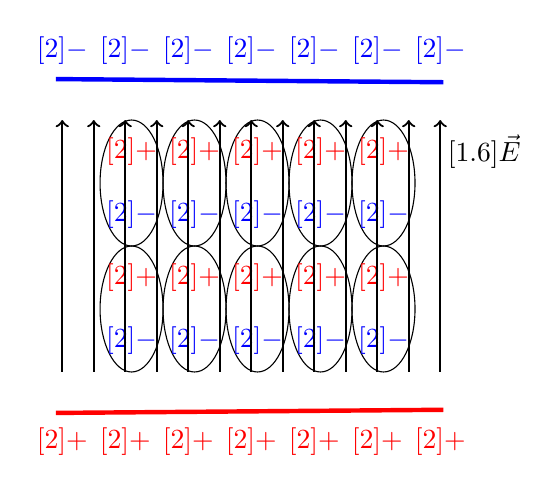
\begin{tikzpicture}[xscale=0.4,yscale=0.4]
    \draw[black] (-4,-2) ellipse (1 and 2);
    \node[blue] at (-4,-3) {$\Scale[2]{-}$};
    \node[red] at (-4,-1) {$\Scale[2]{+}$};
    \draw[black] (-4,2) ellipse (1 and 2);
    \node[blue] at (-4,1) {$\Scale[2]{-}$};
    \node[red] at (-4,3) {$\Scale[2]{+}$};
    \draw[black] (-2,-2) ellipse (1 and 2);
    \node[blue] at (-2,-3) {$\Scale[2]{-}$};
    \node[red] at (-2,-1) {$\Scale[2]{+}$};
    \draw[black] (-2,2) ellipse (1 and 2);
    \node[blue] at (-2,1) {$\Scale[2]{-}$};
    \node[red] at (-2,3) {$\Scale[2]{+}$};
    \draw[black] (0,-2) ellipse (1 and 2);
    \node[blue] at (0,-3) {$\Scale[2]{-}$};
    \node[red] at (0,-1) {$\Scale[2]{+}$};
    \draw[black] (0,2) ellipse (1 and 2);
    \node[blue] at (0,1) {$\Scale[2]{-}$};
    \node[red] at (0,3) {$\Scale[2]{+}$};
    \draw[black] (2,-2) ellipse (1 and 2);
    \node[blue] at (2,-3) {$\Scale[2]{-}$};
    \node[red] at (2,-1) {$\Scale[2]{+}$};
    \draw[black] (2,2) ellipse (1 and 2);
    \node[blue] at (2,1) {$\Scale[2]{-}$};
    \node[red] at (2,3) {$\Scale[2]{+}$};
    \draw[black] (4,-2) ellipse (1 and 2);
    \node[blue] at (4,-3) {$\Scale[2]{-}$};
    \node[red] at (4,-1) {$\Scale[2]{+}$};
    \draw[black] (4,2) ellipse (1 and 2);
    \node[blue] at (4,1) {$\Scale[2]{-}$};
    \node[red] at (4,3) {$\Scale[2]{+}$};
    \draw[black, thick, ->] (-6.2,-4) -- (-6.2,4);
    \draw[black, thick, ->] (-5.2,-4) -- (-5.2,4);
    \draw[black, thick, ->] (-4.2,-4) -- (-4.2,4);
    \draw[black, thick, ->] (-3.2,-4) -- (-3.2,4);
    \draw[black, thick, ->] (-2.2,-4) -- (-2.2,4);
    \draw[black, thick, ->] (-1.2,-4) -- (-1.2,4);
    \draw[black, thick, ->] (-0.2,-4) -- (-0.2,4);
    \draw[black, thick, ->] (0.8,-4) -- (0.8,4);
    \draw[black, thick, ->] (1.8,-4) -- (1.8,4);
    \draw[black, thick, ->] (2.8,-4) -- (2.8,4);
    \draw[black, thick, ->] (3.8,-4) -- (3.8,4);
    \draw[black, thick, ->] (4.8,-4) -- (4.8,4);
    \draw[black, thick, ->] (5.8,-4) -- (5.8,4);
    \node[black] at (7.2,3) {$\Scale[1.6]{\vec{E}}$};
    \draw[red, ultra thick] (-6.4,-5.3) -- (5.9,-5.2);
    \draw[blue, ultra thick] (-6.4,5.3) -- (5.9,5.2);
    \node[blue] at (-6.2,6.2) {$\Scale[2]{-}$};
    \node[blue] at (-4.2,6.2) {$\Scale[2]{-}$};
    \node[blue] at (-2.2,6.2) {$\Scale[2]{-}$};
    \node[blue] at (-0.2,6.2) {$\Scale[2]{-}$};
    \node[blue] at (1.8,6.2) {$\Scale[2]{-}$};
    \node[blue] at (3.8,6.2) {$\Scale[2]{-}$};
    \node[blue] at (5.8,6.2) {$\Scale[2]{-}$};
    \node[red] at (-6.2,-6.2) {$\Scale[2]{+}$};
    \node[red] at (-4.2,-6.2) {$\Scale[2]{+}$};
    \node[red] at (-2.2,-6.2) {$\Scale[2]{+}$};
    \node[red] at (-0.2,-6.2) {$\Scale[2]{+}$};
    \node[red] at (1.8,-6.2) {$\Scale[2]{+}$};
    \node[red] at (3.8,-6.2) {$\Scale[2]{+}$};
    \node[red] at (5.8,-6.2) {$\Scale[2]{+}$};
\end{tikzpicture}
\end{figure}

\end{frame}

\begin{frame}{Dielectrics}

So the dielectric sets up its own electric field that acts in opposition to the electric field of the capacitor. But recall that the voltage difference between the two plates separated a distance $d$ is
\begin{equation*}
    \left| \Delta V \right| = \int \vec{E} \cdot d\vec{\ell} = E \cdot d 
\end{equation*}

So if the electric field gets weaker, the voltage difference between the capacitor plates gets correspondingly weaker. Now recall the definition of capacitance:
\begin{equation*}
    C = \frac{Q}{\Delta V}
\end{equation*}

Charge $Q$ is fixed and $\Delta V$ decreases. So the capacitance increases!

\end{frame}

\begin{frame}{Gauss's Law in Dielectrics}

With dielectrics, we make one substitution to Gauss's law: $\epsilon_o \to \epsilon = \kappa \epsilon_o$. So Gauss's law becomes
\begin{equation*}
    \oint \vec{E} \cdot d\vec{A} = \frac{Q_{\text{enc}}}{\epsilon_o} \quad \to \quad \oint \vec{E} \cdot d\vec{A} = \frac{Q_{\text{enc}}}{\epsilon}
\end{equation*}

\end{frame}

\begin{frame}{Worked Example --- Finding the Capacitance of Concentric Spheres}

$\blacktriangleright$ Consider a spherical shell of radius $a$, nested within a larger spherical shell of radius $b$. The space between them is filled with a dielectric with dielectric constant $\kappa$.

\begin{figure}
\centering
\includegraphics[height=0.5\textheight]{figures/two.png}
\end{figure}

Find the capacitance of this arrangement.

\end{frame}

\begin{frame}{Worked Example --- Finding the Capacitance of Concentric Spheres}

\textit{Solution.} Let's start with the definition of capacitance:
\begin{equation*}
    C = \frac{Q}{\Delta V}
\end{equation*}

And assume a charge of $+Q$ on the inner electrode and $-Q$ on the outer electrode:

\begin{figure}
\centering
\includegraphics[height=0.36\textheight]{figures/twol.png}
\end{figure}

Now we just need to find the potential difference $\Delta V$ between the two electrodes. And for that, we need to integrate over the electric field!

\end{frame}

\begin{frame}{Worked Example --- Finding the Capacitance of Concentric Spheres}

To find the electric field, we can apply Gauss's law, which reads
\begin{equation*}
    \oint \vec{E} \cdot d\vec{A} = \frac{Q_{\text{enc}}}{\epsilon}
\end{equation*}

We want to find the electric field in between the electrodes (for $r$ such that $a < r < b$).

\end{frame}

\begin{frame}{Worked Example --- Finding the Capacitance of Concentric Spheres}

Consider a spherical Gaussian surface of radius $r$, such that $a < r < b$:

\begin{figure}
\centering
\includegraphics[height=0.36\textheight]{figures/tree.png}
\end{figure}

This Gaussian surface encloses the charge $+Q$. Moreover, its surface area is $4\pi r^2$. All pertinent symmetry arguments hold. So solving for the electric field gives
\begin{gather*}
    \oint \vec{E} \cdot d\vec{A} = \frac{Q_{\text{enc}}}{\epsilon} \implies E \left( 4\pi r^2 \right) = \frac{+Q}{\kappa \epsilon_o} \implies E = \frac{Q}{4\pi \kappa \epsilon_o r^2}
\end{gather*}

\end{frame}

\begin{frame}{Worked Example --- Finding the Capacitance of Concentric Spheres}

We can integrate this electric field to find the magnitude of the potential difference $\Delta V$ between the electrodes:
\begin{align*}
    \big| \Delta V \big| &= \int \vec{E} \cdot d\vec{\ell} \\
    &= \int_a^b \left( \frac{Q}{4\pi \kappa \epsilon_o r^2} \right)\ dr \\
    &= \frac{Q}{4\pi\kappa\epsilon_o} \int_a^b \frac{dr}{r^2} \\
    &= \frac{Q}{4\pi\kappa\epsilon_o} \left( -\frac{1}{r} \right) \bigg|_{a}^{b} \\
    &= \frac{Q}{4\pi\kappa\epsilon_o} \left( \frac{1}{a} - \frac{1}{b} \right)
\end{align*}

\end{frame}

\begin{frame}{Worked Example --- Finding the Capacitance of Concentric Spheres}

Again, the definition of capacitance is
\begin{equation*}
    C = \frac{Q}{\Delta V}
\end{equation*}

Substituting for the voltage difference $\Delta V$, we have
\begin{equation*}
    C = \frac{\cancel{Q}}{\frac{\cancel{Q}}{4\pi\kappa\epsilon_o} \left( \frac{1}{a} - \frac{1}{b} \right)} = \boxed{\frac{4\pi\kappa\epsilon_o}{\left( \frac{1}{a} - \frac{1}{b} \right)}} \blacktriangleleft
\end{equation*}

\end{frame}

\begin{frame}{Charging RC Circuits}

A \emph{charging} RC circuit might look like this:

\begin{figure}[H]
\centering
\begin{circuitikz}
    \draw (0,0) to[american voltage source,l^=$\mathscr{E}$] (0,3);
    \draw (0,3) to[nos] (4,3);
    \draw (4,3) to[resistor,l^=$R$] (4,0);
    \draw (4,0) to[capacitor,l^=$C$] (0,0);
    % \draw (0,0.9) to[resistor,l^=$R_1$,i>=$\textcolor{BLUE}{I_1}$] (0,3);
    % \draw (0,3) to[battery,invert,l^=$V_2$] (0,4);
    % \draw (3,0) to[resistor,l^=$R_2$,i>=$\textcolor{BLUE}{I_2}$] (3,4);
    % \draw (6,0) to[battery,invert,l^=$V_3$,i>=$\textcolor{BLUE}{I_3}$] (6,2.4);
\end{circuitikz}
\end{figure}

The capacitor starts out initially uncharged. At $t=0$, the switch is closed and the capacitor charges according to
\begin{equation*}
    Q(t) = Q_{\text{final}} \left( 1 - e^{-t/RC} \right)
\end{equation*}

\end{frame}

\begin{frame}{Charging RC Circuits --- A Mini Derivation}

The figure below shows an RC circuit at some time $t > 0$. The emf source $\mathscr{E}$ is charging the capacitor $C$ through the resistor $R$. A current $I$ flows through the resistor as charge $Q$ builds up on the capacitor:

\vspace{-1em}

\begin{figure}[H]
\centering
\begin{circuitikz}[scale=0.8]
    \draw (0,0) to[american voltage source,l^=$\mathscr{E}$] (0,3);
    % \draw (0,3) to[switch] (4,3);
    % \draw (1,3) to[short,*-*,i>=$I$] (1,3) node[label={[font=\small]below:$\textcolor{RED}{\text{Bottom Junction}}$}] {} to (3,3);
    \draw (0,3) to (1.5,3);
    \draw (1.5,3) to[short,*-*,i>=$I$] (2.5,3); 
    \draw (2.5,3) to (4,3);
    \draw (4,3) to[resistor,l^=$R$] (4,0);
    \draw (4,0) to[capacitor,l^=$C$] (0,0);
    % \draw (0,0.9) to[resistor,l^=$R_1$,i>=$\textcolor{BLUE}{I_1}$] (0,3);
    % \draw (0,3) to[battery,invert,l^=$V_2$] (0,4);
    % \draw (3,0) to[resistor,l^=$R_2$,i>=$\textcolor{BLUE}{I_2}$] (3,4);
    % \draw (6,0) to[battery,invert,l^=$V_3$,i>=$\textcolor{BLUE}{I_3}$] (6,2.4);
\end{circuitikz}
\end{figure}

\vspace{-1em}

If we apply Kirchhoff's Voltage Law to the circuit above, then conservation of energy requires
\begin{equation*}
    \underbrace{\hspace{1em}\mathscr{E}\hspace{1em}}_{\Delta V_{\text{emf}}} + \underbrace{\hspace{1em}-I(t) R\hspace{1em}}_{\Delta V_R} + \underbrace{\hspace{1em} -\frac{Q(t)}{C} \hspace{1em}}_{\Delta V_C} = 0
\end{equation*}

\end{frame}

\begin{frame}{Charging RC Circuits --- A Mini Derivation}

So Kirchhoff's Voltage Law gave us
\begin{gather*}
    \mathscr{E} - I(t) R - \frac{Q(t)}{C} = 0 \quad \implies \quad I(t) R + \frac{Q(t)}{C} = \mathscr{E}
\end{gather*}

The capacitor is charging, so $I = +\frac{dQ}{dt}$, which means we can express the above equation as an ordinary differential equation for the charge $Q(t)$ on the capacitor:
\begin{equation*}
    \frac{dQ(t)}{dt} + \frac{Q(t)}{RC} = \frac{\mathscr{E}}{R}
\end{equation*}

Solving this differential equation gives
\begin{equation*}
    \boxed{Q(t) = C \mathscr{E} \left( 1 - e^{-t/RC} \right) = Q_{\text{final}} \left( 1 - e^{-t/RC}\right)}
\end{equation*}

This is the same equation that's on the equation sheet and it's all we need!

\end{frame}

\begin{frame}{Charging RC Circuits}

So the charge on the capacitor is
\begin{equation*}
    Q(t) = C \mathscr{E} \left( 1 - e^{-t/RC} \right)
\end{equation*}

What if we want the current in the circuit? Current is just the time-derivative of charge:
\begin{equation*}
    I(t) = +\frac{dQ(t)}{dt} = \frac{\mathscr{E}}{R} e^{-t/RC} = I_{\text{init}} e^{-t/RC}
\end{equation*}

What if we want the potential difference across the resistor $\Delta V_R$? That just comes from Ohm's law:
\begin{equation*}
    \Delta V_R (t) = I(t) R = \mathscr{E} e^{-t/RC}
\end{equation*}

What if we want the potential difference across the capacitor $\Delta V_C$? That just comes from the definition of capacitance:
\begin{equation*}
    \Delta V_C (t) = \frac{Q(t)}{C} = \mathscr{E} \left( 1 - e^{-t/RC} \right)
\end{equation*}

\end{frame}

\begin{frame}{Discharging RC Circuits}

A \emph{discharging} RC circuit might look like this:

\begin{figure}[H]
\centering
\begin{circuitikz}
    \draw (0,0) to[capacitor,l^=$C$] (0,3);
    \draw (0,3) to[nos] (4,3);
    \draw (4,3) to[resistor,l^=$R$] (4,0);
    \draw (4,0) to (0,0);
    % \draw (0,0.9) to[resistor,l^=$R_1$,i>=$\textcolor{BLUE}{I_1}$] (0,3);
    % \draw (0,3) to[battery,invert,l^=$V_2$] (0,4);
    % \draw (3,0) to[resistor,l^=$R_2$,i>=$\textcolor{BLUE}{I_2}$] (3,4);
    % \draw (6,0) to[battery,invert,l^=$V_3$,i>=$\textcolor{BLUE}{I_3}$] (6,2.4);
\end{circuitikz}
\end{figure}

The capacitor starts out initially charged. At $t=0$, the switch is closed and the capacitor discharges according to
\begin{equation*}
    Q(t) = Q_{\text{initial}} e^{-t/RC}
\end{equation*}

\end{frame}

\begin{frame}{Discharging RC Circuits --- A Mini Derivation}

The figure below shows an RC circuit at some time $t > 0$. A capacitor $C$ is discharging itself through the resistor $R$. A current $I(t)$ flows through the resistor as charge $Q(t)$ leaves the capacitor:

\vspace{-1em}

\begin{figure}[H]
\centering
\begin{circuitikz}[scale=0.8]
    \draw (0,0) to[capacitor,l^=$C$] (0,3);
    % \draw (0,3) to[nos] (4,3);
    \draw (4,3) to[resistor,l^=$R$] (4,0);
    \draw (4,0) to (0,0);
    % \draw (0,3) to[switch] (4,3);
    % \draw (1,3) to[short,*-*,i>=$I$] (1,3) node[label={[font=\small]below:$\textcolor{RED}{\text{Bottom Junction}}$}] {} to (3,3);
    \draw (0,3) to (1.5,3);
    \draw (1.5,3) to[short,*-*,i>=$I$] (2.5,3); 
    \draw (2.5,3) to (4,3);
\end{circuitikz}
\end{figure}

\vspace{-1em}

If we apply Kirchhoff's Voltage Law to the circuit above, then conservation of energy requires
\begin{equation*}
    \underbrace{\hspace{1em} \frac{Q(t)}{C} \hspace{1em}}_{\Delta V_C} + \underbrace{\hspace{1em}-I(t) R\hspace{1em}}_{\Delta V_R} = 0
\end{equation*}

\end{frame}

\begin{frame}{Discharging RC Circuits --- A Mini Derivation}

So Kirchhoff's Voltage Law gave us
\begin{equation*}
    \frac{Q(t)}{C} - I(t) R = 0 \quad \implies \quad -I(t) R + \frac{Q(t)}{C} = 0
\end{equation*}

The capacitor is discharging, so $I=-\frac{dQ}{dt}$, which means we can express the above equation as an ordinary differential equation for the charge $Q(t)$ on the capacitor:
\begin{equation*}
    \frac{dQ(t)}{dt} + \frac{Q(t)}{RC} = 0 
\end{equation*}

Solving this differential equation gives
\begin{equation*}
    \boxed{Q(t) = Q_{\text{initial}} e^{-t/RC}}
\end{equation*}

This is the same equation that's on the equation sheet and it's all we need!

\end{frame}

\begin{frame}{Discharging RC Circuits}

So the charge on the capacitor is
\begin{equation*}
    Q(t) = Q_{\text{initial}} e^{-t/RC}
\end{equation*}

What if we want the current in the circuit? Current is just the time derivative of charge (negative here because capacitor is losing charge):
\begin{equation*}
    I(t) = -\frac{dQ(t)}{dt} = \frac{Q_{\text{init}}}{RC} e^{-t/RC} = I_{\text{init}} e^{-t/RC}
\end{equation*}

What if we want the potential difference across the resistor $\Delta V_R$? That just comes from Ohm's law:
\begin{equation*}
    \Delta V_R (t) = I(t) R = \frac{Q_{\text{init}}}{C} e^{-t/RC}
\end{equation*}

What if we want the potential difference across the capacitor $\Delta V_C$? That just comes from the defintion of capacitance:
\begin{equation*}
    \Delta V_C (t) = \frac{Q(t)}{C} = \frac{Q_{\text{init}}}{C} e^{-t/RC}
\end{equation*}

\end{frame}

\begin{frame}{AC Circuits}

An AC signal varies with time, such as that shown below:

\begin{figure}[H]
\centering
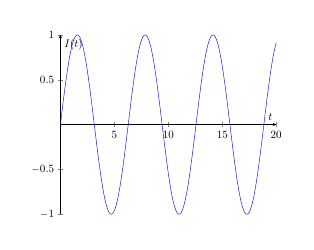
\begin{tikzpicture}[scale=0.4]
\begin{axis}[axis lines = center, xlabel = $t$, ylabel = {$I(t)$}]
\addplot[domain=0:20, samples=200, color=blue] {sin(deg(x))};
\end{axis}
\end{tikzpicture}
\end{figure}

\begin{center}
(In practice, the signal need not be sinusoidal, but that's what we'll be dealing with.)
\end{center}

We need two parameters to describe an AC signal: the amplitude (either $V_o$ or $I_o$) and the frequency $f$ (measured in \textbf{hertz} (Hz): $\SI{1}{\hertz} = \SI{1}{\text{cycle}\per\second}$). Note that the angular frequency $\omega$ and the frequency $f$ are related via
\begin{equation*}
    \omega = 2\pi f
\end{equation*}

\end{frame}

\begin{frame}{Root-Mean-Square Values}

Suppose a current is given as $I(t) = I_{\text{max}} \cos{(\omega t)}$. Its root-mean square value is
\begin{align*}
    I_{\text{rms}} &= \sqrt{\left( I^2 \right)_{\text{mean}}} = \sqrt{\left( I_{\text{max}}^2 \cos^2{\left(\omega t\right)}\right)_{\text{mean}}} = \sqrt{\frac{I_{\text{max}}^2}{2}} = \frac{I_{\text{max}}}{\sqrt{2}}
\end{align*}

In general, for a quantity that varies with time as a sinusoidal function, the rms value is the maximum value divided by $\sqrt{2}$.

The expressions for resistor circuits are pretty much still the same:
\begin{gather*}
    P = I \left( \Delta V \right) \quad \implies \quad P_{\text{mean}} = I_{\text{rms}} \left( \Delta V_{\text{rms}} \right) \\
    P = I^2 R \quad \implies \quad P_{\text{mean}} = I_{\text{rms}}^2 R \\
    \Delta V = I R \quad \implies \quad \Delta V_{\text{rms}} = I_{\text{rms}} R
\end{gather*}

\end{frame}

\begin{frame}{Resistors in AC Circuits}

Consider the circuit shown, with input signal $V(t) = V_o \cos{(\omega t)}$

\begin{figure}[H]
\centering
\begin{circuitikz}
    \draw (0,0) to[vsourcesin,l^=$V(t)$] (0,2);
    \draw (0,2) to (3,2);
    \draw (3,2) to[resistor,l^=$R$] (3,0);
    \draw (3,0) to (0,0);
\end{circuitikz}
\end{figure}

Ohm's law still holds, and the current in the circuit is
\begin{equation*}
    I(t) = \frac{V(t)}{R} = \frac{V_o}{R} \cos{(\omega t)} = I_o \cos{(\omega t)}
\end{equation*}

\end{frame}

\begin{frame}{Capacitors in AC Circuits}

Consider the circuit shown, with input signal $V(t) = V_o \cos{(\omega t)}$

\begin{figure}[H]
\centering
\begin{circuitikz}
    \draw (0,0) to[vsourcesin,l^=$V(t)$] (0,2);
    \draw (0,2) to (3,2);
    \draw (3,2) to[C,l^=$C$] (3,0);
    \draw (3,0) to (0,0);
    % \draw (0,0.9) to[resistor,l^=$R_1$,i>=$\textcolor{BLUE}{I_1}$] (0,3);
    % \draw (0,3) to[battery,invert,l^=$V_2$] (0,4);
    % \draw (3,0) to[resistor,l^=$R_2$,i>=$\textcolor{BLUE}{I_2}$] (3,4);
    % \draw (6,0) to[battery,invert,l^=$V_3$,i>=$\textcolor{BLUE}{I_3}$] (6,2.4);
\end{circuitikz}
\end{figure}

Note that the charge on the capacitor is
\begin{equation*}
    Q = C V = C \left( V_o \cos{(\omega t)} \right)
\end{equation*}

Then the current in the circuit is
\begin{equation*}
    I(t) = \frac{d}{dt} \overbrace{\left( C V_o \cos{(\omega t)} \right)}^{Q(t)} = -\underbrace{V_o \omega C}_{I_o} \sin{(\omega t)} = -I_o \sin{\left( \omega t \right)}
\end{equation*}

Note that the current goes like $\sin{(\omega t)}$ and the voltage goes like $\cos{(\omega t)}$ --- these are \emph{out of phase}!

\end{frame}

\begin{frame}{Capacitors in AC Circuits}

Observe that $I_o = V_o \omega C$. So let's define a quantity $X$ such that 
\begin{equation*}
    V_o = X I_o
\end{equation*}

This sort of resembles Ohm's Law! And in fact, $X$ is known as \emph{reactance} and it plays the role of resistance for a capacitor:
\begin{equation*}
    X = \frac{1}{\omega C}
\end{equation*}

Reactance is small for large $\omega$ and large for small $\omega$. This is a way of quantifying the statement ``with low-frequency (DC-like) input, capacitors prevent charge flow.''

\end{frame}

\begin{frame}{Resistors and Capacitors Together in AC Circuits}

Now consider the following circuit:

\begin{figure}[H]
\centering
\begin{circuitikz}
    \draw (0,0) to[vsourcesin,l^=$V(t)$] (0,3);
    \draw (0,3) to (3,3);
    \draw (3,3) to[R,l^=$R$] (3,1.2);
    \draw (3,1.2) to[C,l^=$C$] (3,0);
    \draw (3,0) to (0,0);
\end{circuitikz}
\end{figure}

Now we'll define the \emph{impedance}, $Z$, as follows:
\begin{equation*}
    Z = \sqrt{R^2 + X^2} = \sqrt{R^2 + \frac{1}{\left( \omega C \right)^2}}
\end{equation*}

The impedance is the total effective resistance (we can't simply add $X$ and $R$). The rms current through the circuit comes from
\begin{equation*}
    V_{\text{rms}} = I_{\text{rms}} Z
\end{equation*}

where $V_{\text{rms}}$ is the input signal.

\end{frame}

\begin{frame}{Low-Pass Filters}

The output voltage is measured across the capacitor on a low-pass filter:

\begin{figure}[H]
\centering
\begin{circuitikz}
    \draw (0,0) to[vsourcesin,l^=$V_{\text{in}}$] (0,3);
    \draw (0,3) to[R,l^=$R$] (3,3);
    \draw (3,3) to[C,l_=$C$,v^<=$V_{\text{out}}$] (3,0);
    \draw (3,0) to (0,0);
\end{circuitikz}
\end{figure}

The gain is the ratio of the output voltage to the input voltage:
\begin{gather*}
    \text{Gain} = \frac{V_{\text{out, rms}}}{V_{\text{in, rms}}} = \frac{V_{C, \text{ rms}}}{V_{\text{in, rms}}} = \frac{I_{\text{rms}}\ X_C}{I_{\text{rms}}\ Z} = \frac{X_C}{Z} \\
    \implies \text{Gain} = \frac{\left( \frac{1}{\omega C} \right)}{\sqrt{R^2 + \left( \frac{1}{\omega C} \right)^2}} = \frac{1}{\sqrt{\left( \omega R C \right)^2 + 1}}
\end{gather*}

\end{frame}

\begin{frame}{High-Pass Filters}

The output voltage is measured across the resistor on a high-pass filter:

\vspace{-0.8em}

\begin{figure}[H]
\centering
\begin{circuitikz}
    \draw (0,0) to[vsourcesin,l^=$V_{\text{in}}$] (0,3);
    \draw (0,3) to[C,l^=$C$] (3,3);
    \draw (3,3) to[R,l_=$R$,v^<=$V_{\text{out}}$] (3,0);
    \draw (3,0) to (0,0);
\end{circuitikz}
\end{figure}

The gain is the ratio of the output voltage to the input voltage:
\begin{gather*}
    \text{Gain} = \frac{V_{\text{out, rms}}}{V_{\text{in, rms}}} = \frac{V_{R, \text{ rms}}}{V_{\text{in, rms}}} = \frac{I_{\text{rms}}\ R}{I_{\text{rms}}\ Z} = \frac{R}{Z} \\
    \implies \text{Gain} = \frac{R}{\sqrt{R^2 + \left( \frac{1}{\omega C} \right)^2}} = \frac{\omega R C}{\sqrt{\left( \omega R C \right)^2 + 1}}
\end{gather*}

\end{frame}

\end{document}
